\section{Catalogue des solutions et tests effectués}
\subsection{Pré-étude des micro-capsules}

Les micro-capsules sont fabriqué à partir de verre borosilicate 3.3 (voir Annexe \ref{pdf:borosilicate}), ce type 
de verre est souvent utilisé pour la verrerie de laboratoire. En effet, il comporte une 
très bonne résistance aux chocs thermique du faite de son faible coefficient de dilatation. 
De plus, il est résistant à de nombreux produits chimiques.
Néanmoins, son comportement mécanique peut s'avéré fragile en particulier pour de faibles
épaisseurs (voir \cite{report_borosilicate}).

\vspace{0.3cm}

\begin{figure}[H]
    \centering
    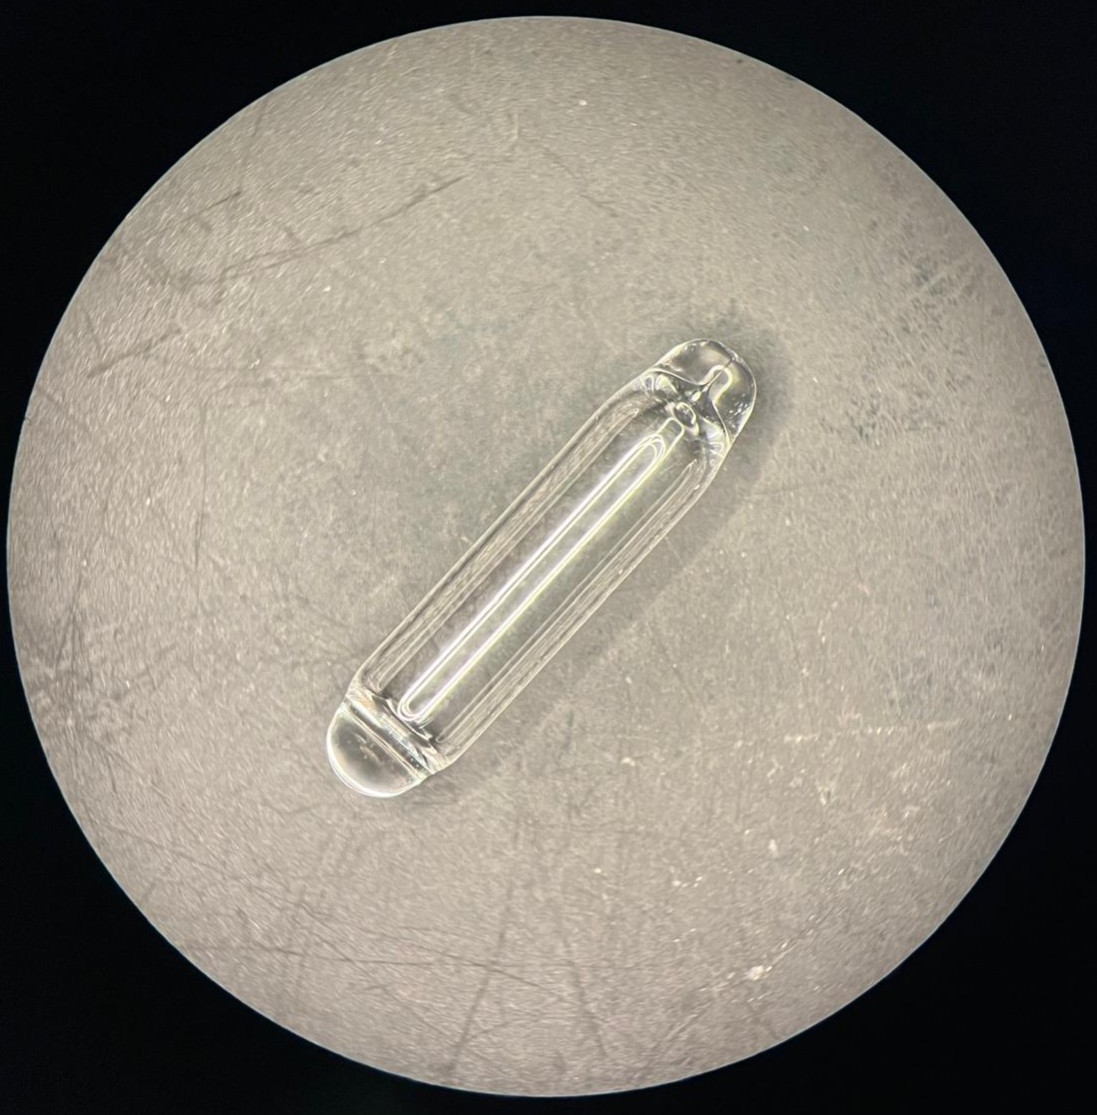
\includegraphics[width=7cm]{Images/Illustrations/CDH/Micro-capsule.jpg}
    \label{fig:microcapsule_loupe}
    \caption{Observation d'une micro-capsule avec une loupe binoculaire}
\end{figure}

Les micro-capsules seront fermée à terme par une entreprise externe à l'aide d'une machine laser permettant de sceller le verre.
Cependant pour le moment, par soucis de simplicité, les micro-capsules sont fermée manuellement grâce à une 
perceuse à colonne et un chalumeau.

\begin{figure}
    \centering
    \begin{subfigure}[b]{0.4\textwidth}
        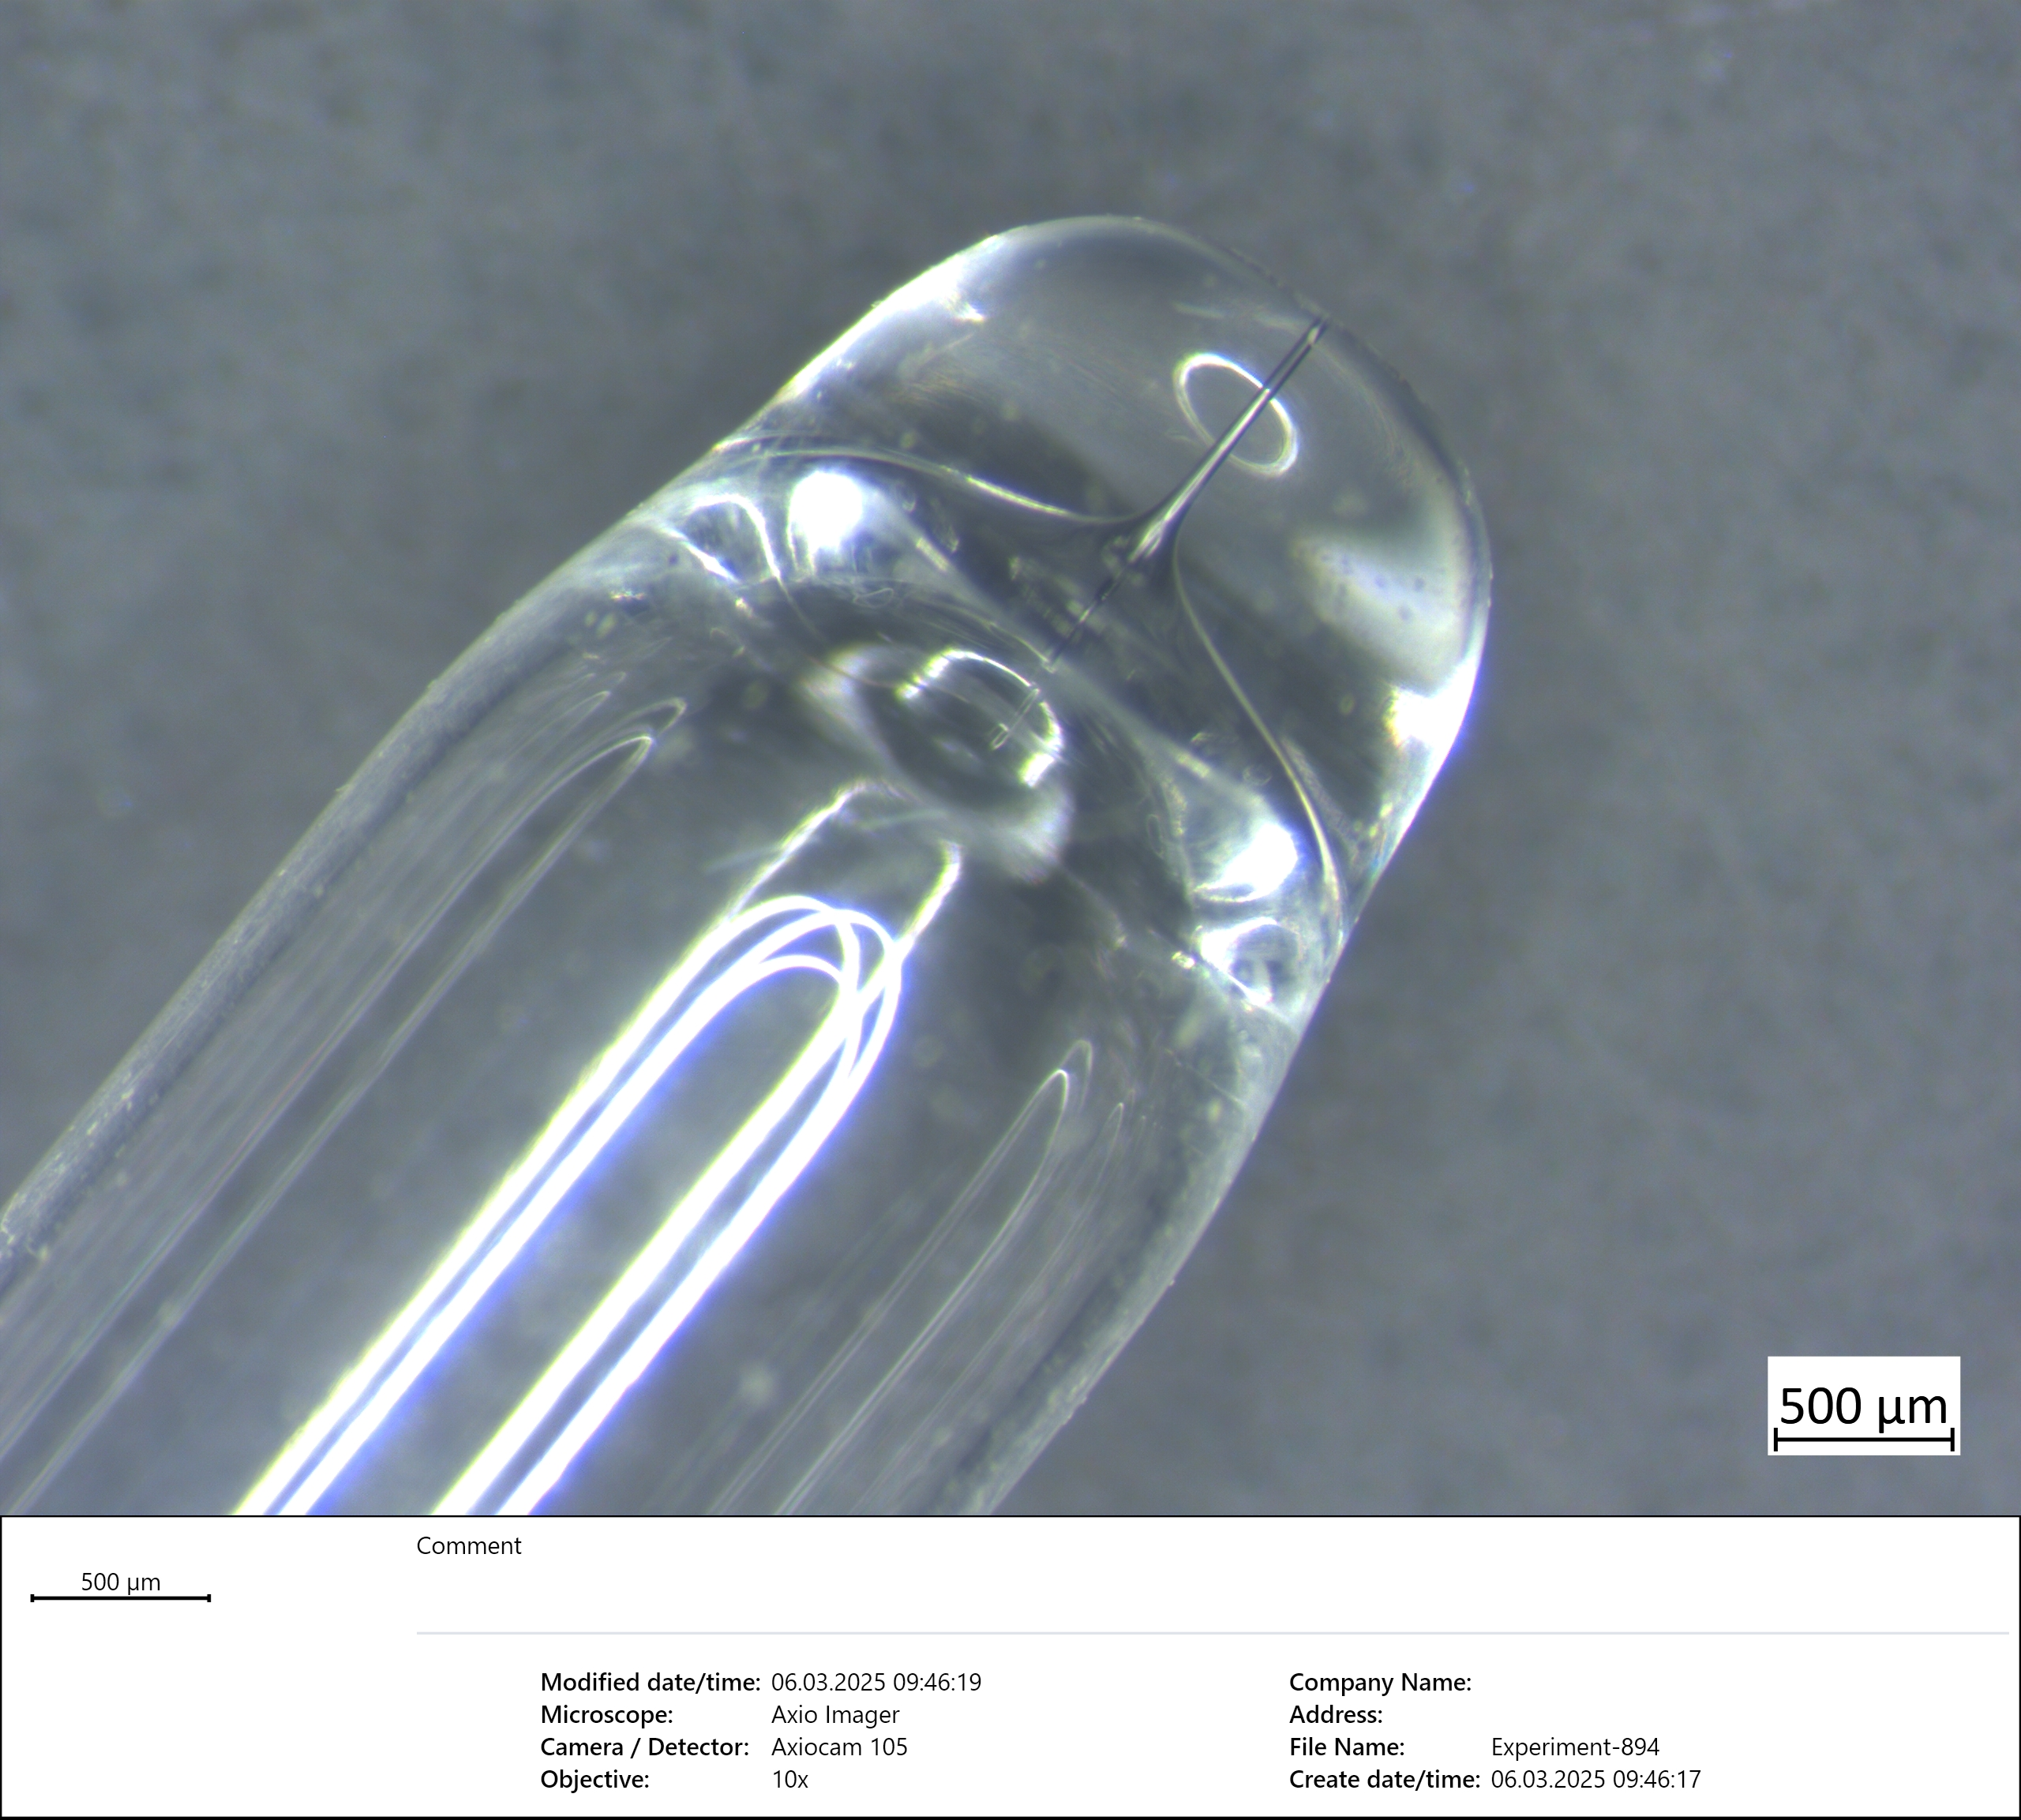
\includegraphics[width=6cm]{Images/Illustrations/CDH/MicroCapsule_trou.jpg}
        \caption{Micro-capsule mal fermée observé au microscope}
        \label{fig:trou_microcapsule}
    \end{subfigure}
    \begin{subfigure}[b]{0.4\textwidth}
        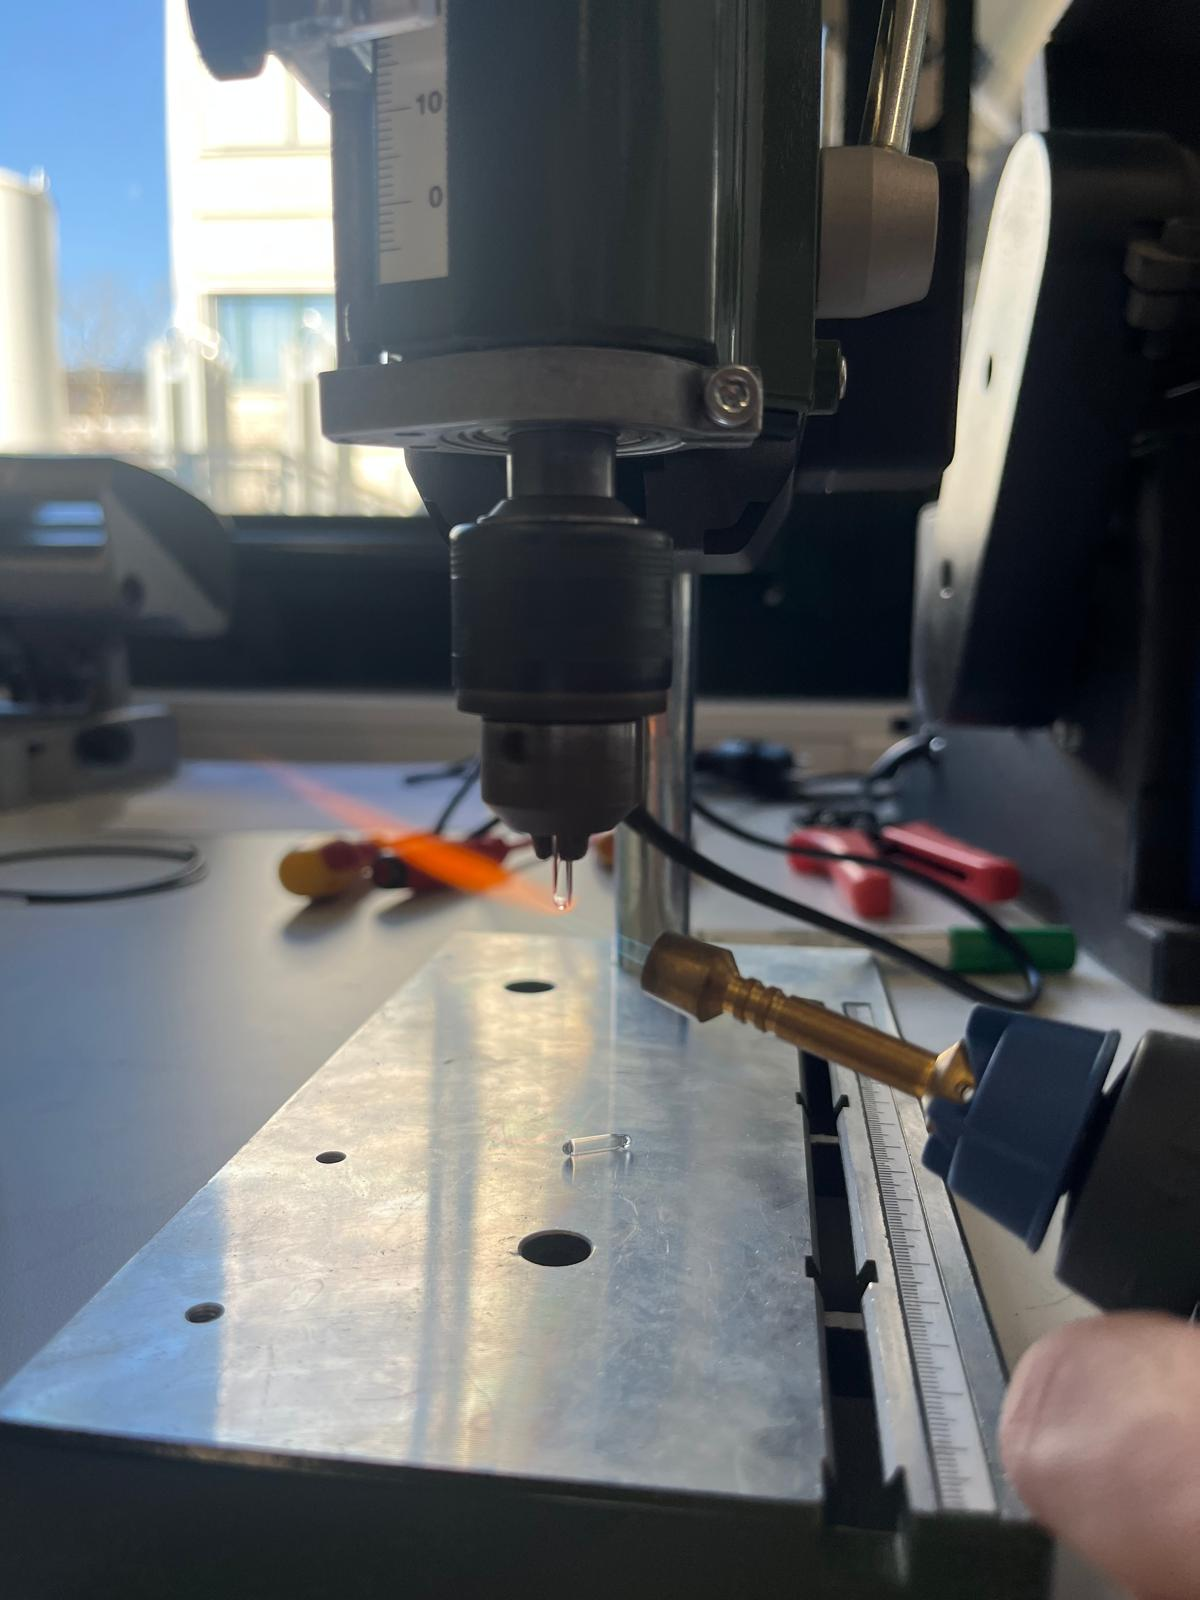
\includegraphics[width=6cm]{Images/Illustrations/CDH/Fermeture_capsule.jpg}
        \caption{Fermeture d'une micro-capsule avec le chalumeau}
        \label{fig:chalumeau}
    \end{subfigure}
    \caption{Fermeture manuel des micro-capsules}
    \label{fig:fermeture_microcapsule}
\end{figure}




\subsection{Liste des solutions envisagées}
\subsubsection{Canon à azote}
\paragraph{Principe de la solution}
L'idée de cette solution est de placer la micro-capsule dans un tube, puis de la soumettre à une pression d'azote élevée.
Ce qui aura pour effet de propulser la micro-capsule contre le fond du réacteur.

\paragraph{Tests et simulations}
Prototype réalisé en impression 3D (voir figure \ref{fig:proto_canon}).
Des tests ont été effectués avec une pression de 5 bar dans le tube.

\begin{figure}[H]
    \centering
    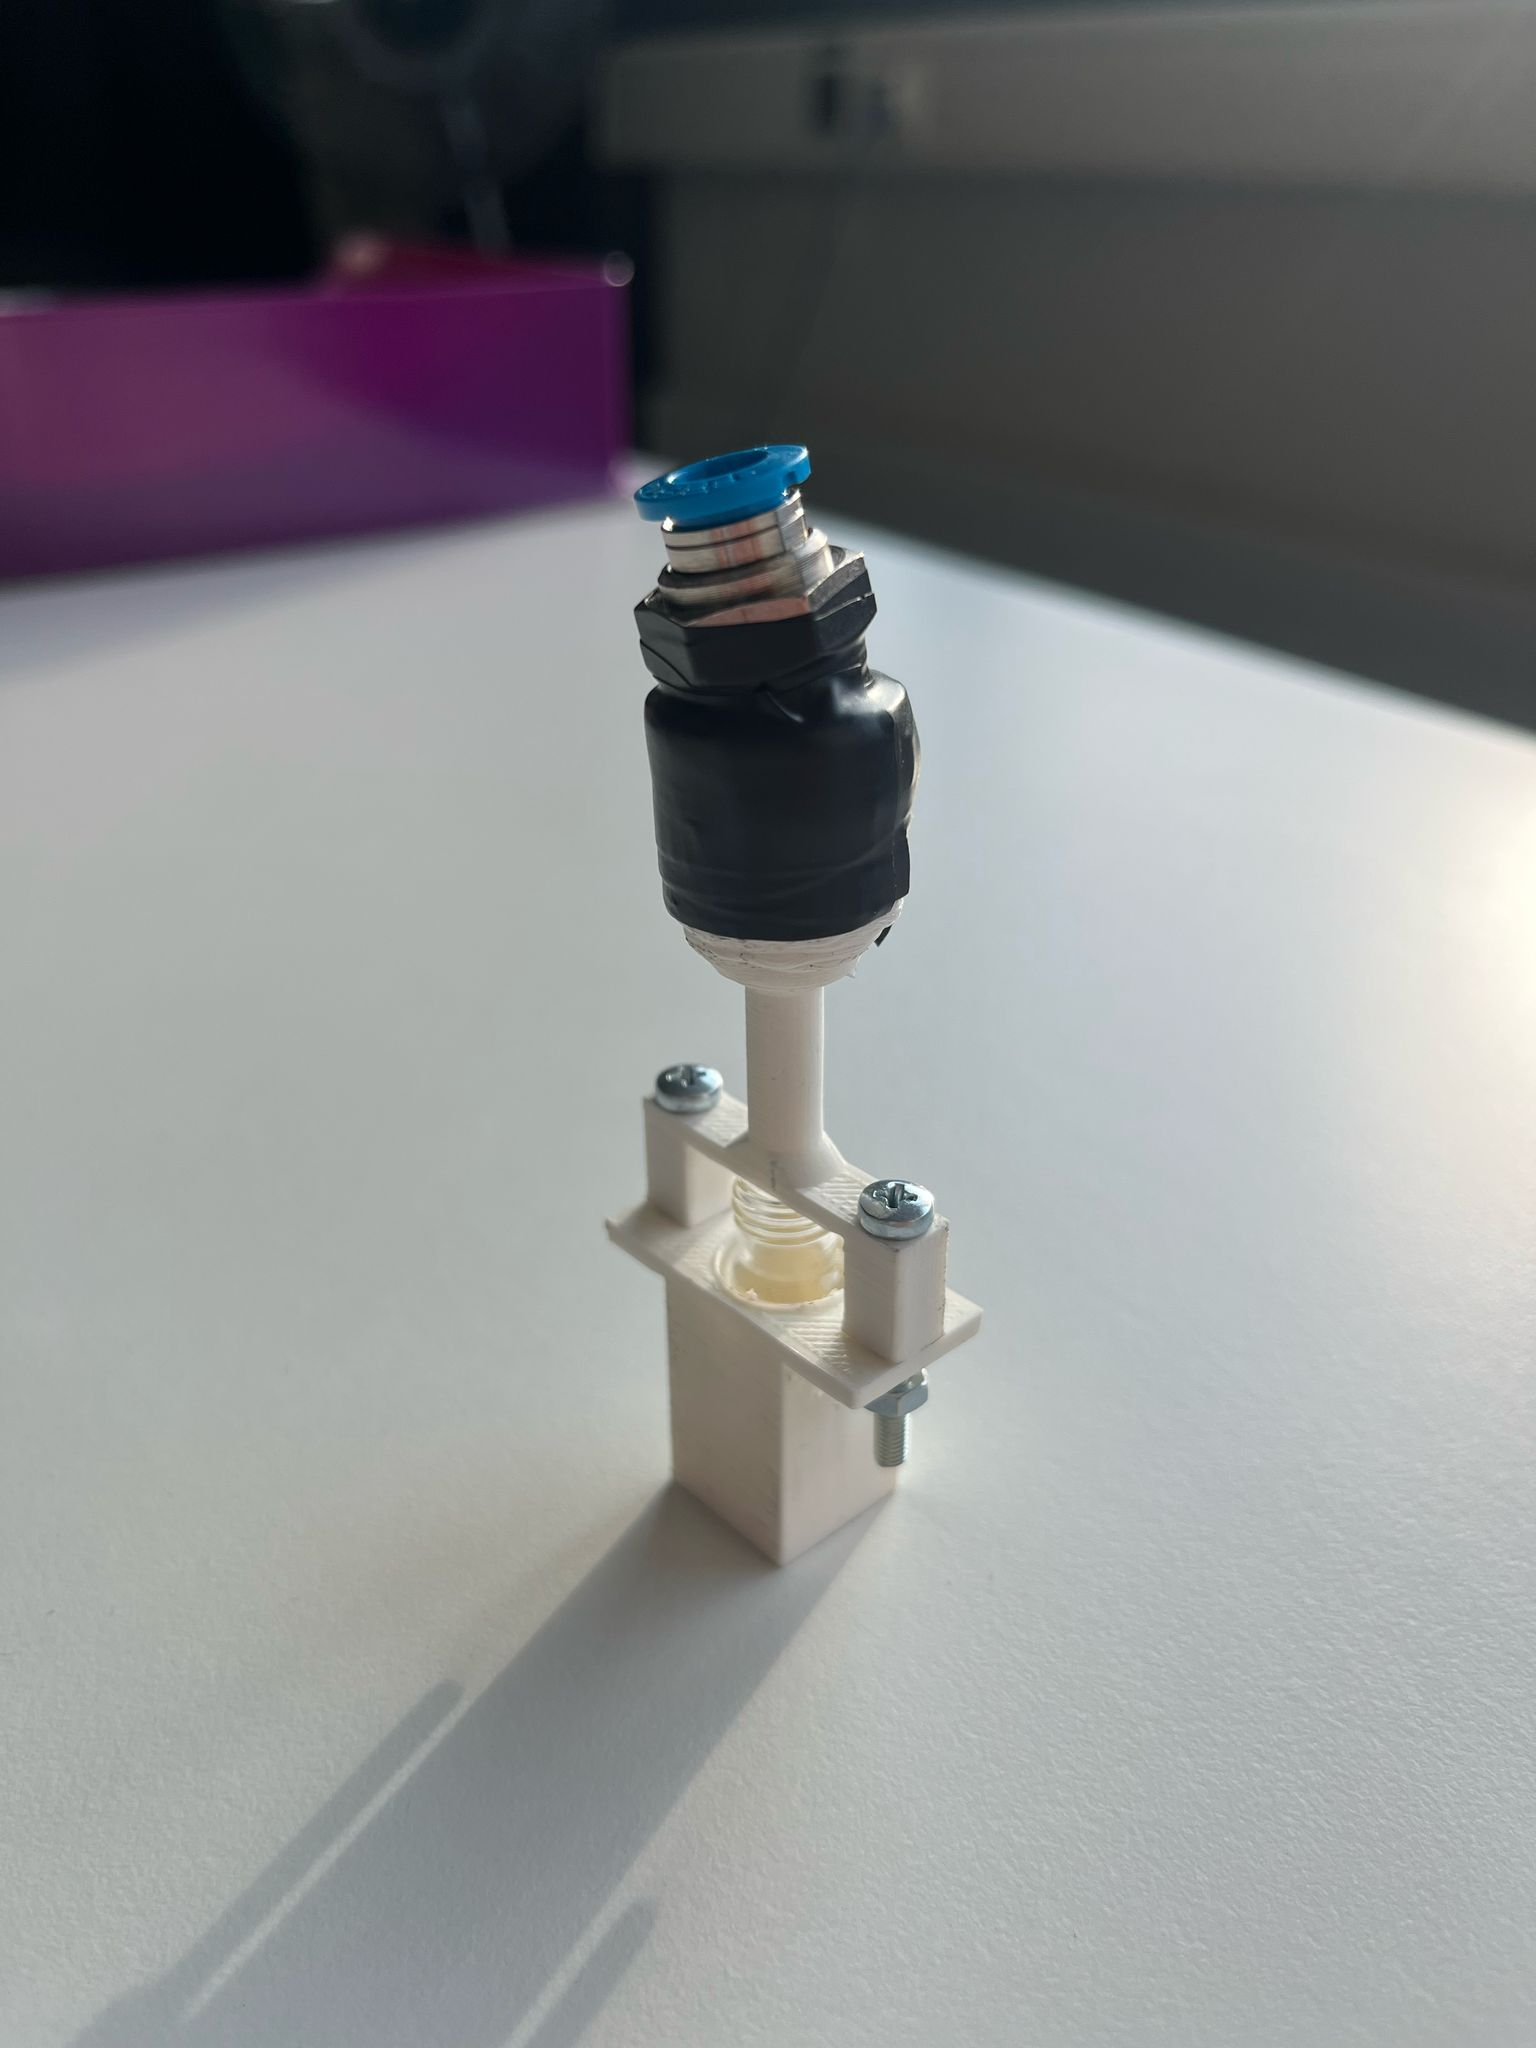
\includegraphics[width=6cm]{Images/Illustrations/CDH/Proto_canon.jpg}
    \caption{Prototype du canon à azote}
    \label{fig:proto_canon}
\end{figure}

\paragraph{Conclusion}
En conclusion, lors des essais réalisé, la micro-capsule ne s'est pas brisée pour des pressions inférieures à 10 bar.
En outre, après discutions au-près des chimistes, le risque de cross-contamination est trop élevé, dû aux éclats de verre et à certains réactifs très volatiles.
Enfin, la complexité de la mise en place de cette solution pour une application de pick and place est trop importante. 
Ce qui rend cette solution non viable pour le projet.

\subsubsection{Implosion de la capsule}
\paragraph{Principe de la solution}
Le principe de cette solution est de placer tout les réacteurs contenant des micro-capsules dans une chambre que
l'on va soumettre à une forte pression. Cette pression devrait provoquer l'implosion des micro-capsules.

\paragraph{Tests et simulations}
Une chambre de mise sous pression utilisé pour de précédents tests à été réutilisé.


\begin{table}[H]
    \centering
    \begin{tabular}{|l|l|}
    \hline
    \rowcolor[HTML]{C1EB5F} 
    \multicolumn{1}{|c|}{\cellcolor[HTML]{C1EB5F}\textbf{Avantages}} &
      \multicolumn{1}{c|}{\cellcolor[HTML]{E4AAAB}\textbf{Inconvenients}} \\ \hline
    \begin{tabular}[c]{@{}l@{}}Cassage des capsules effectué \\ directement dans le réacteur.\end{tabular} &
      \begin{tabular}[c]{@{}l@{}}Nécessite une pression assez\\ élevée.\end{tabular} \\ \hline
    \begin{tabular}[c]{@{}l@{}}Peu ou pas de cross-contamination \\ si implosion contrôlée.\end{tabular} &
      \begin{tabular}[c]{@{}l@{}}Simulation et comportement\\ plus complexe.\end{tabular} \\ \hline
    \end{tabular}
    \caption{Avantages et inconvénients du cassage par pression}
    \label{tab:AvIncPression}
    \end{table}

\paragraph{Conclusion}


\subsubsection{Actionneur mécanique}
\paragraph{Principe de la solution}

\paragraph{Tests et simulations}

\paragraph{Conclusion}

\subsubsection{Fréquence de résonance}
\paragraph{Principe de la solution}

\paragraph{Tests et simulations}

\paragraph{Conclusion}


\subsection{Critères et choix de la solution}
